\documentclass{jsarticle}

\usepackage[dvipdfmx]{graphicx}
\usepackage{multicol}
\usepackage{here}
\usepackage{geometry}
\geometry{left=25mm,right=25mm,top=10mm,bottom=20mm}

\title{情報通信プロジェクト G班企画書}
\author{13EC602 郭柏辰, 14EC004 飯田頌平, 14EC552 陳玉皓, 14EC602 劉宇航}

\begin{document}

	\maketitle
	
	%\begin{multicols}{2}
	
		\section{企画の目的}
		
			% 背景
			既存の天気予報は都市毎にしか見ないものであったり、
			雨雲の動きを生データで実況するものが多く、
			気象予報士でもない一般人が特定の位置の天気を予報するには向いていない。
			
			% 目的
			そのため、センサを活用して局地的な天気を予測できる
			IoTデバイスに需要があると考えられる。
		
		\section{構成}
		
			% 問題設定
			局地的な情報を計測する必要があるため、
			センサは持ち運びができるものでなくてはならない。
			
			センサが測定したデータを取り出す部品も、同様にコンパクトである必要がある。
			
			% 使用機材
			そこで、データ取得を行う部品にRaspberryPiを採用する。
			RaspberryPiは名刺ほどの小型のコンピュータであり、
			MicroSDカードにシステムやデータを保存する。
			
			RaspberryPiはGPIO端子を通してI2C(Inter Integrated Circuit)接続を行えるため、
			I2Cに対応したセンサであるBME-280を用いて、温度・湿度・気圧を計測する。
			
			こうして小型の部品を活用することで、どこにでも天気予報機を持ち運んで
			天候のデータを測定することができる。
			
			測ったデータから天気予報を行うには、ニューラルネットワーク\cite{Schmidhuber}という
			アルゴリズムを採用する。
			
			RaspberryPiはLinuxベースのOSで動いているため、
			Pythonプログラムで実装したニューラルネットワークを使って予測を行える。
			
			予測結果は、RaspberryPiのGPIO端子に接続するタイプの
			小型ディスプレイを通してユーザに伝えられるようにする。
		
			以上のことから、構成部品をまとめたものを下に示す。
		
			\begin{center}
				\begin{table}[H]
				  \centering
				  \caption{構成部品一覧}
				  \begin{tabular}{|c|c|r|} \hline
				    種別 & 名称 & 値段\   \\ \hline \hline
				    マイコン & RaspberryPi3 ModelB & 5.600円(a) \\
				    MicroSDカード & SanDisk Ultra 40MB/s 8GB & 798円(b) \\
				    温湿度・気圧センサ & BME-280 モジュール & 1,080円(a) \\
				    ディスプレイ & AE-AQM0802 モジュール & 700円(a) \\
				    オス-オスジャンパ & 10cm20本セット & 180円(a) \\
				    オス-メスジャンパ & 15cm(赤)10本セット & 220円(a) \\
				    ブレッドボード & BB801 & 200円(a) \\ \hline \hline
				     &                 合計 & 8,778円 \\ \hline
				  \end{tabular}
				\end{table}
				{\scriptsize 価格は(a)秋月電子(b)amazon調べ}
			\end{center}
		
		\section{内部仕様}
		
			\subsection{ブロック構成図・回路図}
			
				ブロック構成図兼回路図を図\ref{fig:circuit}に示す。
			
				\begin{figure}[htbp]
				  \begin{center}
				    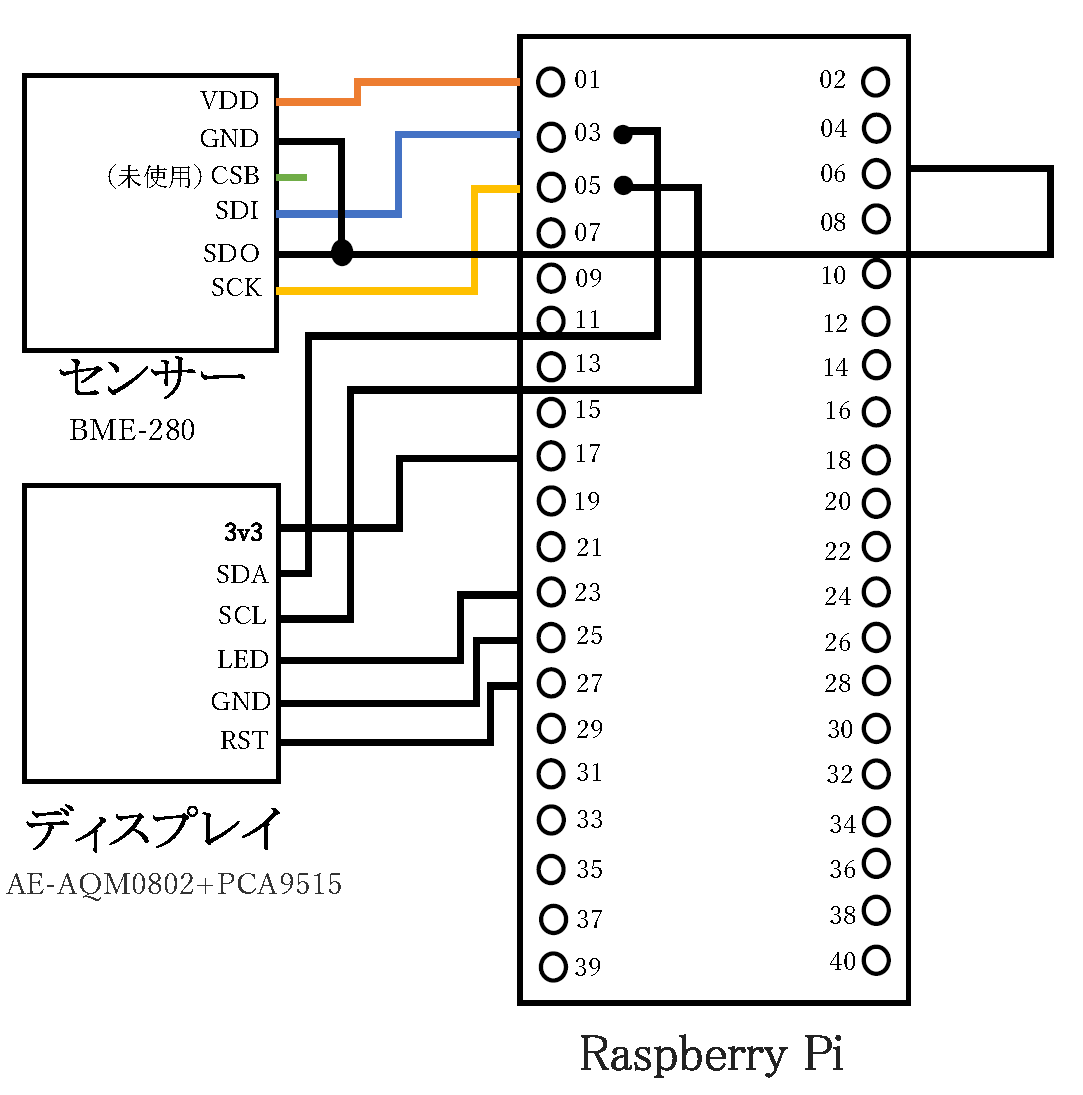
\includegraphics[clip,width=7.0cm]{img/circuit}
				    \caption{ブロック構成図兼回路図}
				    \label{fig:circuit}
				  \end{center}
				\end{figure}
				
				RaspberryPiにはI2Cでセンサとディスプレイが接続されている。
				センサおよびディスプレイはブレッドボード上に配置される。
				
		
			\subsection{ソフトウェア}
			
				\subsubsection{OS}
				
					RaspberryPiを動かすOSには、Raspbianを採用する。
					これはRaspberryPiが公式にサポートしているOSであり、
					Ubuntuベースで作られているため、
					bashを用いて通常のLinuxのようにソフトウェアを動かせるためだ。
					
				\subsubsection{センサ読み取り}
				
					センサが取得したデータを読み取るソフトには、
					センサ・モジュールの販売元である
					SwitchScienceが提供しているプログラムを用いる。
					読み取りプログラムはPythonでラップされており、
					Python上のstr(文字列)形式でデータを取得することができる。
					さらにこのコードを改変して、読み取ったデータを
					天気予報用のプログラムに送信するようにする。
					
					また、定期的なデータの取得にはbashコマンドのcrontabというものを用いる。
					これによって、一時間毎にデータを読み取るコマンドを自動的に実行できる。
					
				\subsubsection{天気予報}
				
					天気予報を行うプログラムとして、
					Pythonでニューラルネットワークを実装したコードを用いる。
					
					Pythonは深層学習用のライブラリを多数有しており、
					ニューラルネットワークを用いたプログラムの実装に向いているためだ。
					
					実装にあたって、深層学習用ライブラリのKerasを採用する。
					Kerasはバックエンドのライブラリに数値計算の処理を任せており、
					勾配法の実装などの詳細な点を無視しながら
					比較的簡単にニューラルネットワークを実装できる。
					
					今回用いるものはLSTM\cite{Hochreiter}と呼ばれるモデルだが、
					これは時系列の情報を学習することができ、
					通常のニューラルネットワークよりも
					時間の変化による予測値の変化に敏感になるためだ。
					
					一般的に、ニューラルネットワークによる予測には、
					事前に学習用データを用いてネットワークの訓練を行う必要がある。
					学習用データには、気象庁が用意しているCSVデータを採用する。
					これは不要な情報が多々含まれているため、
					Pythonプログラムによって必要な情報だけを抽出する。
					
					抽出する情報は、一時間あたりの温度・湿度・気圧・降水量の4項目で、
					これらを一年分用意する。
					降水量についてはしきい値を取り、一定量の降水量があったときに
					雨天であると判定し、ブール値でフラグを立てるように変換する。
					
					そうして生成されたデータを逐次的にLSTMに入力し、
					誤差逆伝播法\cite{Le}のアルゴリズムによって
					天気予報に適したモデルを生成する。
					天気予報モデルは、センサから得た温度・湿度・気圧の3次元のデータに基いて、
					未来の降水確率を出力する。
					
					%天気予報用モデルはふたつのネットワークからなる。
					%第一のネットワークは、回帰によって未来のデータを予測する。
					%具体的には、温度・湿度・気圧の3次元のデータについて、
					%観測時点のデータとその12時間前までのデータを入力することで、
					%次の12時間分の各データを予測する。
					%第二のネットワークは、予測されたデータを用いて、
					%未来の各時点での降水確率を出力する。
					
				\subsubsection{ディスプレイ}
				
					採用したディスプレイAE-AQM0802は、RaspberryPiからbashコマンドで動作させることができる。
					Pythonのsubprocessモジュールからbashを操作することで、
					間接的にPythonプログラム上からディスプレイの操作ができる。
			
		\section{外部仕様}
		
			% 完成予想図と使い方
			
			本デバイスの使用方法は、以下の手順に則る。
			
			\begin{enumerate}
				\item デバイスの電源を入れて、起動する
				\item デバイスを適当な観測箇所に設置する
				\item ディスプレイに出力された天気予報を確認する
			\end{enumerate}
			
			センサによる測定を行う上で、屋外での動作が見込まれているが、
			予算の都合上、雨よけのケースや携帯型のバッテリーを不採用にしたので、
			実際の運用では窓の近くに設置する形が想定される。
			
			ディスプレイの出力値は、単純に確率を数値で表したものと、
			その確率をどう判断すべきかの目安となる文字列を表すことにする。
			これによって、ユーザは傘を持っていくかどうかという、
			もっとも重要な情報を即座に判断できるようになる。
	
	\begin{thebibliography}{9}
	  \bibitem{Schmidhuber} Schmidhuber, Jürgen. "Deep learning in neural networks: An overview." Neural networks 61 (2015): 85-117.
	  \bibitem{Hochreiter} Hochreiter, Sepp, and Jürgen Schmidhuber. "Long short-term memory." Neural computation 9.8 (1997): 1735-1780.
	  \bibitem{Le} LeCun, Y., Boser, B., Denker, J.S., Henderson, D., Howard, R.E., Hubbard, W., \& Jackel, L.D. (1990). Handwritten digit recognition with a back-propagation network.Advances in Neural Information Processing Systems, 2, 396–404, Morgan Kaufman.
	\end{thebibliography}
		
	%\end{multicols}

\end{document}